\section{derivata}

Il potenziale gravitazionale generato dalla terra nello spazio, in un punto
a distanza $r$ dal suo centro è dato da:
\[
U(r) = -\frac{GM}{r}
\]
dove $M$ è la massa della terra e $G$ è la costante di gravitazione universale.
La funzione $U(r)$ non è affatto lineare. Se però consideriamo il
campo gravitazionale per i punti in prossimità della
superficie terrestre, ci aspettiamo un comportamento approssimativamente
lineare. Proviamo a esplicitare questa idea.

Supponiamo di trovarci ad altezza $h$ dalla superficie terrestre. Ci
troveremo allora a distanza $R+h$ dal centro della terra. Si avrà allora:
\[
  U(R+h) = -GM\frac{1}{R+h}.
\]
Osserviamo ora che si ha
\begin{align*}
  \frac{1}{R+h}
  & = \frac{1}{R} + \frac{1}{R+h} - \frac{1}{R}
   = \frac 1 R + \frac{R-(R+h)}{R(R+h)} \\
  & = \frac 1 R - \frac{h}{R(R+h)} \\
  & = \frac 1 R - \frac{h}{R^2} - \frac{h}{R(R+h)} + \frac{h}{R^2} \\
  & = \frac 1 R - \frac{h}{R^2} - \frac{hR - h(R + h)}{R^2(R+h)} \\
  & = - \frac{h}{R^2} + \frac 1 R + \frac{h^2}{R^2(R+h)}.
\end{align*}
Dunque si avrà
\begin{align*}
  U(R+h) &= \frac{GM}{R^2} h - \frac{GM}{R} + \omega(h)\\
  &= g h + C + \omega(h)
\end{align*}
dove $g = GM/R^2$, $C$ è una costante (irrilevante perché il
potenziale può essere definito a meno di una costante) e
$\omega(h)$ è una funzione con la proprietà $\omega(h)/h\to 0$
per $h\to 0$. Dunque se $h$ è molto piccolo rispetto a $R$, il termine
$\omega(h)$ è trascurabile rispetto al termine $gh$ (anche se entrambi
tendono a zero per $h\to 0$). Questo giustifica
l'utilizzo della formula
semplificata:
\[
U_0(h) = gh
\]
da cui l'energia potenziale $E = mgh$
se abbiamo una massa $m$ ad una altezza $h$ sulla superficie terrestre.

\begin{figure}
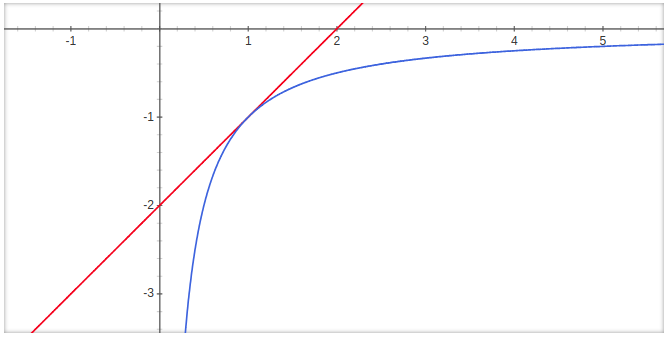
\includegraphics[width=0.49\textwidth]{derivata_00.png}\hfill%
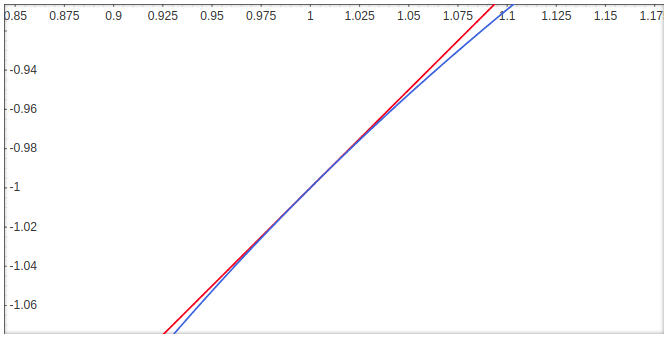
\includegraphics[width=0.49\textwidth]{derivata_01.png}
\label{fig:derivata}
\caption{Il grafico del potenziale gravitazionale terrestre.
Sull'asse delle $x$ la distanza dal centro della terra in raggi terrestri.
Sull'asse delle $y$ il potenziale gravitazionale con unità $C=GM/R$.
La pendenza della retta tangente al grafico della curva per $x=R$ è $g=GM/R^2$.
Nella figura di destra un ingrandimento in un intorno del raggio terrestre:
si nota come il grafico del potenziale risulta quasi indistinguibile dal
grafico della retta tangente.}
\end{figure}

Quello che abbiamo fatto è un procedimento di \emph{linearizzazione}%
\mymargin{linearizzazione}%
\index{linearizzazione}. 
Il campo gravitazionale è descritto da una funzione non lineare: $-GM/r$.
Ma quando ci restringiamo a un piccolo intervallo di valori di $r$ 
(i valori di $r$ vicini ad $R$, il raggio della terra) tale funzione 
risulta quasi indistinguibile, a meno di una costante, dalla funzione 
lineare $gh$ se $r=R+h$.
Le funzioni lineari sono molto più semplici da trattare ed è quindi conveniente, 
se rimaniamo sulla superficie terrestre, utilizzare quest'ultima formula per 
il potenziale gravitazionale.
Il grafico della funzione lineare che meglio approssima il grafico di una 
funzione si chiama \emph{retta tangente}%
\mymargin{retta tangente}%
\index{retta!tangente}. 
Il suo coefficiente angolare, $g$ nel nostro esempio, si chiama \emph{derivata}%
\mymargin{derivata}%
\index{derivata}.

Una volta introdotte le derivate vedremo che quello che abbiamo
determinato è la formula:
\[
U(R+h) = U(R) + U'(R) h + \omega(h).
\]

\begin{definition}[derivata]
\mymark{***}%
Sia $A\subset \RR$, $f\colon A \to \RR$, 
$x_0\in A$ un punto di accumulazione di $A$.
Diremo che la funzione $f$ è \emph{derivabile} nel punto $x_0$ se esiste
ed è finito il limite:
\[
  \lim_{h\to 0} \frac{f(x_0+h) - f(x_0)}{h}.
\]
In tal caso denoteremo con $f'(x_0)$ il valore di tale limite che chiameremo
\emph{derivata}%
\mymargin{derivata}%
\index{derivata} della funzione $f$ nel punto $x_0$.

Se $B$ è l'insieme dei punti di accumulazione di $A$ in cui $f$ risulta essere derivabile, risulta quindi definita la funzione derivata $f'\colon B \to \RR$.

Una funzione $f$ si dice essere derivabile se è derivabile in ogni punto del suo dominio.
Se $C\subset A$ la funzione $f$ si dice essere \emph{derivabile su $C$} se è derivabile in ogni punto dell'insieme $C$ (cioè se $C\subset B$).

Notazioni alternative per denotare la derivata di una funzione:
\[
  f' = Df = \frac{d}{dx} f = \frac{df}{dx}.
\]

La definizione di derivata si estende formalmente identica 
alle funzioni di variabile complessa e/o a valori complessi.
La derivata di una funzione a valori complessi è
a sua volta a valori complessi.
\end{definition}

Il rapporto
\[
\frac{f(x_0+h) - f(x_0)}{h}
\]
si chiama \emph{rapporto incrementale}%
\mymargin{rapporto incrementale}%
\index{rapporto!incrementale}. In effetti cambiando variabile e ponendo $x=x_0+h$ si può scrivere
\[
\frac{f(x_0+h) - f(x_0)}{h}
= \frac{f(x) - f(x_0)}{x-x_0}
= \frac{\Delta f}{\Delta x}
\]
che risulta essere il rapporto dell'incremento della funzione $f$ (a volte denotato con $\Delta f$) rispetto all'incremento corrispondente della variabile $x$ (a volte denotato con $\Delta x$).
Cambiando variabile nel limite, per $h\to 0$ si avrà $x\to x_0$
e quindi
\[
 f'(x_0) = \lim_{x\to x_0} \frac{f(x)-f(x_0)}{x-x_0}.
\]

Se $f$ è derivabile nel punto $x_0$
la retta di equazione 
\mymargin{retta tangente}%
\begin{equation}\label{eq:retta_tangente}
  y = f(x_0) + f'(x_0) \cdot (x-x_0)  
\end{equation}
è l'unica retta passante dal punto $(x_0,f(x_0))$ 
con pendenza uguale alla derivata $f'(x_0)$.
Tale retta si chiama \emph{retta tangente}
\index{retta!tangente}%
\index{tangente!al grafico}%
al grafico della funzione $f$ nel punto $(x_0,f(x_0))$.
E' la retta che meglio approssima il grafico di $f$ 
quando $x\to x_0$ nel senso che risulta:
\[
  \lim_{x\to x_0} \frac{f(x) - [f(x_0)+f'(x_0)(x-x_0)]}{x-x_0} = 0
\]
mentre ogni altra retta renderebbe questo limite infinito.

\begin{example}%
\label{ex:derivata_reciproco}%
\mymark{**}%
Si consideri la funzione $f(x) = 1/x$ definita sull'insieme $A = \RR \setminus \ENCLOSE{0}$. Si ha allora per ogni $x\neq 0$:
\[
  f'(x) = \lim_{h\to 0} \frac{\frac{1}{x+h} - \frac{1}{x}}{h}
        = \lim_{h\to 0} \frac{x - (x+h)}{h(x+h)x}
        = \lim_{h\to 0} \frac{-1}{(x+h)x} = -\frac{1}{x^2}.
\]
Risulta quindi che la funzione $1/x$ sia derivabile e la sua derivata è la funzione $-1/x^2$.
\end{example}

\begin{theorem}[continuità delle funzioni derivabili]
\mymark{***}
Se $f$ è derivabile nel punto $x$ allora $f$ è anche continua nel punto $x$.
\end{theorem}
%
\begin{proof}
\mymark{***}
Si ha
\[
  \lim_{h\to 0} f(x+h) - f(x) = \lim_{h\to 0} \frac{f(x+h) - f(x)}{h} \cdot h
  = f'(x) \cdot 0 = 0.
\]
Dunque $f(x+h)\to f(x)$ per $h\to 0$ e quindi $f$ è continua nel punto $x$.
\end{proof}

\begin{example}[funzione continua ma non derivabile]
\mymark{***}
La funzione $f(x) = \abs{x}$ è un esempio di funzione continua ma non
derivabile. E' infatti facile verificare che nel punto $x_0=0$ il
limite destro del rapporto incrementale è $1$ mentre il limite
sinistro è $-1$.

Un altro esempio è la funzione $f(x) = \sqrt{x}$ che è continua ma non
è derivabile nel punto $x_0=0$ perché il limite del rapporto incrementale esiste ma è $+\infty$.
\end{example}



\begin{theorem}[derivata della funzione composta]
\mymark{**}%
Sia $f$ una funzione derivabile nel punto $x_0$
e sia $g$ una funzione derivabile nel punto $f(x_0)$.
Allora la funzione composta $g\circ f$ è derivabile
nel punto $x_0$ e si ha:
\[
  (g\circ f)'(x_0) = g'(f(x_0))\cdot f'(x_0).
\]
\end{theorem}
%
\begin{proof}
\mymark{**}
Consideriamo la funzione
\[
  G(y) =
  \begin{cases}
   \frac{g(y) - g(f(x_0))}{y-f(x_0)} & \text{se $y \neq f(x_0)$},\\
   g'(f(x_0)) & \text{se $y=f(x_0)$}.
  \end{cases}
\]
Si avrà allora
\begin{equation}\label{eq:47439}
 \frac{g(f(x_0+h))-g(f(x_0))}{h}
 = G(f(x_0+h)) \cdot \frac{f(x_0+h)-f(x_0)}{h}
\end{equation}
infatti se $f(x_0+h)\neq f(x_0)$ abbiamo moltiplicato e diviso
per $f(x_0+h) - f(x_0)$ se invece $f(x_0+h)=f(x_0)$ allora anche $g(f(x_0+h))=g(f(x_0))$ e l'uguaglianza è ancora valida perché sia il lato sinistro che il lato destro si annullano (e il valore assegnato a $G$ risulta in tal caso irrilevante).

Chiaramente quando $h\to 0$ il secondo fattore sul lato destro
dell'uguaglianza \eqref{eq:47439}
tende, per definizione, a $f'(x_0)$.
Per quanto riguarda il primo fattore
osserviamo che $G(y)$, per come è stata definita, risulta essere una funzione continua nel punto $y=f(x_0)$ in quanto
\[
\frac{g(y) - g(f(x_0))}{y-f(x_0)} \to g'(f(x_0))
\]
per $y\to f(x_0)$.
Ma anche la funzione $f$ è continua nel punto $x_0$ (in quanto derivabile).
Dunque la funzione composta $G(f(x_0+h))$ è continua nel punto $h=0$.
Risulta quindi che $G(f(x_0+h)) \to G(f(x_0)) = g'(f(x_0))$ per $h\to 0$.
Dunque il lato destro di \eqref{eq:47439} ha limite $g'(f(x_0)) \cdot f'(x_0)$ per $h\to 0$, come volevamo dimostrare.
\end{proof}

\begin{theorem}[derivata della funzione inversa]
\mymark{**}
Sia $f$ una funzione invertibile derivabile in un punto $x_0$ e
supponiamo che la funzione inversa $f^{-1}$ sia continua in $f(x_0)$.
Se $f'(x_0)\neq 0$ allora $f^{-1}$ è derivabile in $f(x_0)$ e vale:
\[
  (f^{-1})'(f(x_0)) = \frac{1}{f'(x_0)}.
\]
Chiamato $y_0 = f(x_0)$ la formula può essere anche scritta nella forma:
\[
  (f^{-1})'(y_0) = \frac{1}{f'(f^{-1}(y_0))}.
\]
Se invece $f'(x_0)=0$ la funzione $f^{-1}$ non è derivabile in $f(x_0)$.
\end{theorem}
%
Osserviamo che 
se $I$ è un intervallo,
e se $f\colon I\to \RR$,
è iniettiva e continua allora $J=f(I)$ è un intervallo
e la funzione inversa $f^{-1}\colon J\to I$
è continua (Esercizio~\ref{ex:inversa_monotona}).
%
\begin{proof}
\mymark{**}
Posto $y_0 = f(x_0)$ consideriamo il rapporto incrementale di $f^{-1}$ nel punto $y_0$:
\[
  \frac{f^{-1}(y) - f^{-1}(y_0)}{y-y_0}.
\]
Per $y\to y_0$ possiamo fare il cambio di variabile
$x=f^{-1}(y)$ in quanto avendo assunto che $f^{-1}$ sia continua in $f(x_0)$ sappiamo che se $y\to y_0$ allora $x = f^{-1}(y)\to f^{-1}(y_0) = x_0$.
Si ha allora per $y\to y_0$ che $x\to x_0$ e,
se $f'(x_0)\neq 0$:
\[
  \frac{f^{-1}(y) - f^{-1}(y_0)}{y-y_0}
  = \frac{x-x_0}{f(x)-f(x_0)}
  = \frac{1}{\frac{f(x)-f(x_0)}{x-x_0}} \to \frac{1}{f'(x_0)}.
\]

Se invece $f'(x_0)=0$ il rapporto incrementale della funzione inversa
ha limite infinito e quindi la funzione inversa non è derivabile in $f(x_0)$.
\end{proof}


\begin{theorem}[operazioni con le derivate]
  \label{th:derivate_operazioni}%
\mymark{***}%
Siano $f$ e $g$ due funzioni derivabili in uno stesso punto $x_0$.
Allora le funzioni $f+g$, $f-g$, $f\cdot g$ e, se $g(x_0)\neq 0$ anche $f/g$ sono funzioni derivabili in $x_0$. Nei punti in cui entrambe le funzioni sono derivabili si ha
\begin{gather*}
  (f+g)' = f' + g', \qquad
  (f-g)' = f' - g', \\
  (f\cdot g)' = f' \cdot g + f g', \qquad
  \enclose{\frac{f}{g}}' = \frac{f'g - fg'}{g^2}.
\end{gather*}
\end{theorem}
%
\begin{proof}
\mymark{***}
Per quanto riguarda la derivata della somma (o della differenza) è sufficiente osservare che il rapporto incrementale della somma (o della differenza) è la somma (o la differenza) dei rapporti incrementali e che il limite della somma (o della differenza) è uguale alla somma (o la differenza) dei limiti.

Calcoliamo la derivata del prodotto $f\cdot g$ nel punto $x_0$. Si ha
\begin{align*}
  \frac{f(x)g(x) - f(x_0)g(x_0)}{x-x_0}
  &= \frac{f(x)(g(x) - g(x_0)) + (f(x)-f(x_0))g(x_0)}{x-x_0}\\
  &= f(x) \frac{g(x)-g(x_0)}{x-x_0} + \frac{f(x)-f(x_0)}{x-x_0} g(x_0).
\end{align*}
Passando al limite per $x\to x_0$ ci ricordiamo che $f(x)\to f(x_0)$ in quanto $f$ è continua in $x_0$ (essendo per ipotesi derivabile). I rapporti incrementali tendono alle derivate e si ottiene quindi il risultato voluto $f(x_0) g'(x_0) + f'(x_0) g(x_0)$.

Per quanto riguarda la derivata del rapporto osserviamo che
posto $h(y)=1/y$ si ha
\[
  \frac{f(x)}{g(x)} = f(x) \cdot h(g(x)).
\]
Dall'esempio~\ref{ex:derivata_reciproco} sappiamo che $h'(y) = -1/y^2$ e dunque
possiamo utilizzare le formule per la derivata del prodotto e la derivata della funzione composta per ottenere:
\begin{align*}
  \enclose{\frac{f}{g}}'(x_0)
  &= \enclose{f \cdot (g\circ h)}'(x_0) \\
  &= f'(x_0) \cdot h(g(x_0)) + f(x_0) \cdot h'(g(x_0))\cdot g'(x_0)\\
  &= \frac{f'(x_0)}{g(x_0)} + f(x_0) \cdot \frac{-1}{g^2(x_0)} g'(x_0)\\
  &= \frac{f'(x_0)g(x_0) - f(x_0)g'(x_0)}{g^2(x_0)}.
\end{align*}
\end{proof}

\begin{table}
  \begin{tabular}{c|c||c|c||c|c}
    $f(x)$ & $f'(x)$ & $f(x)$ & $f'(x)$ & $f(x)$ & $f'(x)$
    \\\hline
    $mx + q$ & $m$ &
    $e^x$ & $e^x$ &
    $\sin x$ & $\cos x$ \\
    $\abs{x}$ & $\frac{x}{\abs{x}}$ &
    $\ln x$ & $\frac 1 x$ &
    $\cos x$ & $-\sin x$ \\
    $x^n$ & $n x^{n-1}$ &
    $\sinh x$ & $\cosh x$ &
    $\arcsin x$ & $\frac{1}{\sqrt{1-x^2}}$ \\
    $x^\alpha$ & $\alpha x^{\alpha -1}$ &
    $\cosh x$ & $\sinh x$ & $\arccos x$ & $-\frac{1}{\sqrt{1-x^2}}$ \\
    $\sqrt[n]{x}$ & $\frac{1}{n\sqrt[n]{x^{n-1}}}$ &
    $\settsinh x$ & $\frac{1}{\sqrt{x^2+1}}$ &
    $\tg x$ & $1+ \tg^2 x$ \\
    $\sqrt{x}$ & $\frac{1}{2\sqrt{x}}$ &
    $\settcosh x$ & $\frac{1}{\sqrt{x^2-1}}$ &
    $\arctg x$ & $\frac{1}{1+x^2}$
  \end{tabular}
  \caption{Derivate delle funzioni elementari}
  \label{tab:derivate}%
\end{table}

\begin{theorem}[derivate delle funzioni elementari]%
\label{th:derivate_elementari}%
\index{derivata!delle funzioni elementari}%
\mymark{**}%
Per $m,q,\alpha \in \RR$, $\alpha \neq 0$, $n\in \NN$, $n\neq 0$
valgono le regole di derivazione riassunte nella
tabella~\ref{tab:derivate}: le funzioni nella colonna
$f(x)$ hanno la derivata riportata nella colonna $f'(x)$.
Le funzioni $f(x)$ sono derivabili nei punti del loro dominio 
in cui la corrispondente espressione $f'(x)$ è ben definita.
In particolare:
la funzione $\sqrt[n]{x}$
non è derivabile in $x=0$,
le funzioni $\arcsin x$ e $\arccos x$ non sono derivabili nei punti $-1$ e $1$,
la funzione $\abs{x}$ non è derivabile in $0$,
la funzione $\settcosh x$ non è derivabile in $1$,
la funzione $\ln x$ è derivabile per ogni $x>0$.
Le funzioni lineari, potenze con base positiva, potenze con esponente intero,
esponenziale, logaritmo, seno, coseno, tangente, arcotangente sono invece derivabili
in tutti i punti in cui sono definite.
\end{theorem}

\begin{proof}
\mymark{**}
Per quanto riguarda le funzioni lineari si ha:
\begin{align*}
(mx+q)' &= \lim_{h\to 0}\frac{m(x+h)+q - (mx+q)}{h} = \lim_{h\to 0} m = m.
\end{align*}
Ricordando che la derivata è un limite e che il limite in un punto dipende 
solo dai valori della funzione in un intorno del punto, 
possiamo affermare che la derivata del valore assoluto $\abs{x}$ 
coincide con la derivata di $x$ cioè $1$ sugli $x>0$ e coincide 
con la derivata di $-x$ sugli $x<0$. Dunque $D \abs{x} = x / \abs{x}$ 
se $x\neq 0$. 
Se $x=0$ i limiti destro e sinistro del rapporto incrementale di $\abs{x}$ 
tendono rispettivamente a $1$ e $-1$ e quindi la derivata non esiste.

Dimostriamo che $Dx^n = n x^{n-1}$ per $n\in \NN$, $n>0$, 
per induzione su $n$. Per $n=1$ abbiamo $x^n=x^1$ è lineare 
e quindi dalla formula precedente $Dx^1 = 1 = 1 \cdot x^0$. 
Supponendo di sapere che $D x^n = n x^{n-1}$ si ha, applicando 
la regola di derivazione del prodotto:
\[
  D x^{n+1} = D x\cdot x^n = 1 \cdot x^n + x \cdot n x^{n-1}
   = x^n + n x^n = (n+1) x^n
\]
dimostrando dunque il passo induttivo.
Ricordando la formula di derivazione del rapporto
possiamo trovare la formula per le potenze con esponente intero negativo:
\[
  D x^{-n} = D \frac{1}{x^n} = \frac{-n x^{n-1}}{x^{2n}}
   = -n x^{n-1-2n} = -n x^{-n-1}.
\]

La derivata della radice $n$-esima si trova con la formula di derivazione della funzione inversa $x^n$, che può essere applicata se $x\neq 0$:
\[
  D \sqrt[n]{x} = \frac{1}{n(\sqrt[n]{x})^{n-1}}
    = \frac{1}{n\sqrt[n]{x^{n-1}}}.
\]
Osserviamo che se $n$ è dispari la formula è valida anche per $x<0$.
La derivata della radice quadrata si ottiene ponendo $n=2$.

Per quanto riguarda la derivata dell'esponenziale
ci riconduciamo ad un limite notevole:
\[
  D e^x = \lim_{h\to 0} \frac{e^{x+h}-e^x}{h}
  = \lim_{h\to 0}\frac{e^x e^h - e^x}{h}
  = \lim_{h\to 0}e^x \frac{e^h - 1}{h}
  = e^x.
\]
La derivata del logaritmo si ottiene come derivata della funzione inversa dell'esponenziale:
\[
  D \ln x = \frac{1}{e^{\ln x}} = \frac{1}{x} \qquad\text{per $x>0$}.
\]
Possiamo quindi calcolare la derivata delle potenze con base positiva e esponente reale qualunque:
\[
D x^\alpha
= D e^{\alpha \ln x}
= e^{\alpha \ln x} D(\alpha \ln x)
= x^\alpha \alpha \frac{1}{x}
= \alpha x^{\alpha -1}.
\]

Per quanto riguarda le funzioni trigonometriche 
$\sin$ e $\cos$ ci ricordiamo del limite notevole
(teorema~\ref{th:limite_notevole_sin})
\[
  \lim_{h\to 0}\frac{\sin h}{h} = 1
\]
da cui si ricava, per $h\to 0$ 
\[
\frac{1-\cos h}{h}
= \frac{1-\cos^2 h}{h\cdot(1+\cos h)}
= \frac{\sin^2 h}{h\cdot (1+\cos h)}
= \frac{\sin h}{h} \cdot \frac{\sin h}{1+\cos h}
\to 1 \cdot \frac{0}{2} = 0.
\]
Applicando le formule di addizione si ha
\begin{align*}
  D \sin x
  &= \lim_{h\to 0}\frac{\sin(x+h)-\sin(x)}{h} \\
  &= \lim_{h\to 0}\frac{\sin(x)\cos(h) + \cos(x)\sin(h) - \sin(x)}{h} \\
  &= \lim_{h\to 0}\Enclose{\sin(x) \frac{\cos h-1}{h} + \cos(x) \frac{\sin h}{h}} 
  = \cos(x).
\end{align*}
e similmente
\begin{align*}
  D \cos x
  &= \lim_{h\to 0}\frac{\cos(x+h)-\cos(x)}{h} \\
  &= \lim_{h\to 0}\frac{\cos(x)\cos(h) - \sin(x)\sin(h) - \cos(x)}{h} \\
  &= \lim_{h\to 0}\cos(x) \frac{\cos h-1}{h} - \sin(x) \frac{\sin h}{h} = -\sin(x)
\end{align*}

La funzioni $\arcsin$ è definita come l'inversa della restrizione della funzione $\sin$ all'intervallo $[-\pi/2, \pi/2]$.
Nell'intervallo aperto $(-\pi/2,$ $\pi/2)$ la funzione $\sin$ ha derivata positiva e dunque risulta che la funzione inversa (che sappiamo essere continua) è derivabile in $(-1,1)$ e la sua derivata è
\[
D\arcsin x
= \frac{1}{\cos(\arcsin x)}
= \frac{1}{\sqrt{1-\sin^2 \arcsin x}}
= \frac{1}{\sqrt{1-x^2}}.
\]
Si ha infatti $\cos y = \sqrt{1-\sin^2 y}$ se $y\in [-\pi/2, \pi/2]$.

Analogamente la funzione $\arccos$ è definita come l'inversa della restrizione di $\cos$ all'intervallo $[0,\pi]$ e si ha quindi,
per $x\in (-1,1)$
\[
D \arccos x
 = \frac{1}{-\sin(\arccos x)}
 = \frac{1}{-\sqrt{1-\cos^2 \arccos x}}
 = -\frac{1}{\sqrt{1-x^2}}.
\]
Si ha infatti $\sin y = \sqrt{1-\cos^2 y}$ se $y\in[0,\pi]$.

Nei punti $x=1$ e $x=-1$ le funzioni $\arcsin$ e $\arccos$ non sono invece derivabili.

Per la funzione tangente possiamo utilizzare la formula di derivazione del rapporto:
\begin{align*}
  D \tg x &= D \frac{\sin x }{\cos x}
   = \frac{\cos x \cdot \cos x - \sin x \cdot (-\sin x)}{\cos^2 x} \\
   &= \frac{\cos^2 x + \sin^2 x}{\cos^2 x}
   = 1 + \tg^2 x = \frac{1}{\cos^2 x}.
\end{align*}
Usando la formula della derivata della funzione inversa si ha
\[
  D \arctg x = \frac{1}{1+\tg^2(\arctg x)}
  = \frac{1}{1+x^2}.
\]

Per quanto riguarda le funzioni iperboliche le derivate di $\sinh$
e $\cosh$ si riconducono immediatamente alla derivata dell'esponenziale,
utilizzando
la definizione~\eqref{eq:sinh_cosh}. Le derivate delle funzioni
inverse $\settsinh$ e $\settcosh$ si ottengono dalla formula per la derivata
della funzione inversa e utilizzando
le relazioni $\cosh x = \sqrt{\sinh^2 x+1}$ e, per $x > 0$,
$\sinh x = \sqrt{\cosh^2 x -1}$:
\begin{align*}
  D \settsinh x &= \frac{1}{\cosh(\settsinh x)}
  = \frac{1}{\sqrt{\sinh^2 (\settsinh x) + 1}} = \frac{1}{\sqrt{x^2+1}}\\
  D \settcosh x &= \frac{1}{\sinh(\settcosh x)}
  = \frac{1}{\sqrt{\cosh^2(\settcosh x)-1}}
  = \frac{1}{\sqrt{x^2-1}}
\end{align*}
\end{proof}

Si noti che le regole di derivazione appena dimostrate 
sono valide anche per le funzioni complesse $z^n$ e $e^z$:
in particolare si ha $D z^n = nz^{n-1}$ per ogni $n\in \ZZ$,
$n\neq 0$ e si ha $D e^z = e^z$ in quanto il limite 
notevole dell'esponenziale è valido anche in campo complesso.
Altre funzioni quali $\sqrt{x}$ 
oppure $\ln x$, non sono univocamente estendibili su $\CC$
e richiedono quindi una teoria a parte. 
Una volta definite, però, si potrebbe verificare 
che anche queste funzioni soddisfano le stesse regole di derivazione 
delle loro restrizioni reali.

\begin{proposition}[trucco di Feynman per le derivate]
  \index{trucco!di Feynman}%
  \index{trucco!di Feynman!per le derivate}%
  \index{Feynman!trucco per le derivate}%
Siano $f_1,\dots, f_n$ funzioni derivabili e siano $\alpha_1,\dots, \alpha_n$ 
esponenti reali. Allora:
  \[
  \enclose{\prod_{k=1}^n f_k^{\alpha_k}}'
  = \prod_{k=1}^n f_k^{\alpha_k} \cdot \sum_{k=1}^n \alpha_k \frac{f_k'}{f_k}.
  \]
\end{proposition}
\begin{proof}
Basta osservare che 
\begin{align*}
  \enclose{\prod_{k=1}^n f_k^{\alpha_k}}'
  &= \sum_{k=1}^n \alpha_k f_k' f_k^{\alpha_k-1} \prod_{j\neq k} f_j^{\alpha_j}
  = \sum_{k=1}^n \alpha_k \frac{f_k'}{f_k} \prod_{j=1}^n f_j^{\alpha_j}.
\end{align*}
\end{proof}
Se ad esempio vogliamo calcolare la derivata della funzione 
\[
 f(x) = \frac{\sqrt{1-x^2}\cdot \ln x}{x\cdot \cos^2 x}
 = (1-x^2)^{\frac 1 2} \cdot \ln x \cdot x^{-1}\cdot (\cos x)^{-2}
\]
otteniamo 
\begin{align*}
  f'(x) 
  &= \frac{\sqrt{1-x^2}\cdot \ln x}{x\cdot \cos^2 x}
  \cdot \Enclose{\frac 1 2 \cdot \frac{-2x}{1-x^2} + \frac{1}{x\ln x} - \frac{1}{x}-2\frac{-\sin x}{\cos x}}\\
  &=\frac{\sqrt{1-x^2}\cdot \ln x}{x\cdot \cos^2 x}
  \cdot \Enclose{-\frac{x}{1-x^2} + \frac{1}{x\ln x} - \frac{1}{x}+2\tg x}.
\end{align*}

